\graphicspath{ {../body/handover_figures/}}
\chapter{WiMAX网络中高速移动用户的基站切换}
\echapter{Handover or High Velocity Mobile Station in WiMAX Networks}
\label{chap_iccs_handover_alogrithm}
本章研究的内容是
如何改善WiMAX网络中高速移动用户基站切换成功率的问题。
首先我们以移动WiMAX网络为例,
对移动用户在通信的过程中,基站切换操作所涉及到的具体流程与信令进行了细致地分析与讨论。
而后,提出并建立了一个切换信令协议交换的概率模型;
并且深入分析了用户的移动速度对切换成功概率的影响。
最后提出了一个用于在不同移动速度下保证切换成功率的自适应前向纠错方案。
该方案使用增加额外的信令保护措施,来确保基站切换过程满足所需的设计要求。


\section{引言}
\esection{Introduction}
\label{section_iccs_handover_algorithm_introduction}
在蜂窝通信网络中,
术语“切换”(handover 或 handoff)是指将一个正在通话或是进行数据传输业务的移动用户从一个通信信道转到另一个通信信道的过程。
通常,出现切换操作的原因有多种。
例如,移动终端物理位置的变化。一个正在通信的用户从一个基站(Base Station,BS)进入到了另一个基站的信号覆盖范围。
为了避免通信中断,这个用户就要进行切换操作:
在断开与当前基站或小区连接的同时,连接上第二个基站,并继续保持通信过程。
还有的时候,用户位于几个基站覆盖域的重叠区域。
此时,如果出现某个基站信号质量比当前服务的基站信号质量好,那么,为了寻求更好的通信质量,
也会进行切换操作。
即使在同一基站有时也会发生切换操作。例如,在某些非CDMA的网络中,
如果一个用户当前使用的信道被邻近小区使用同样信道的用户严重干扰,
那么基站系统也会将此用户的信道切换到同一基站系统的另外一个质量更好的信道上。
还有,如果网络基础架构中存在有宏小区和微小区的设计,在这两种小区之间的信道转变,也称之为切换。
此外,在CMDA网络中,规定一种由于“远近效应”产生的特殊切换过程。
一个用户为避免对其它用户的干扰,即使当前通信质量较好,也会主动地切换到另一个信道,。
基站切换可以在同一网络中的小区之间切换(也被称为微移动性,Micro-mobility),也可以在异构的网络之间切换。
譬如移动设备在无线局域网(WLAN)和3G通信网之间的切换。

本章中所涉及的切换是指用户终端在移动的过程中(从一个地理位置到另一个地理位置,如图\ref{fig:chap_iccs_handover_bs}),系统采用相应的措施来确保用户的通信服务,并且不被中断\cite{Pollini:1996:THD}\cite{Wright:ICMB2007}。

为了能够具体地分析一个基站的切换流程,我们以移动WiMAX的切换协议作为分析的目标。
首先简要介绍一下移动WiMAX网络。
作为3G通信标准之一,WiMAX是一项用于替代有线宽带访问技术如ADSL,提供最后一公里的无线网络接入技术。
它提供一种方便快速的方法来建立无线城域网(WMN)。
这项技术可以对高速数据业务如宽带互联网访问、VoIP、IPTV等高速率应用提供底层的网络技术支持。
它可用来支持在基站与固定、移动或漫游用户终端之间的高速数据连接。
固定WiMAX (IEEE 802.16-2004)的标准中定义了面向连接的媒体访问层(MAC)和基于正交频分复用(OFDM)的物理层协议 \cite{IEEE:802_16D:2005}。
而移动WiMAX(IEEE 802.16e-2005)的标准中还规定了对于移动用户所需的各种MAC层及物理层协议\cite{IEEE:802_16E:2006}。


%%%%%%%%%%%%%%%%%%%%%%%%%%%%%%%%%%%%%%%%%%%%%%%%%%%%%%%%%%%%%%%%%%%%%
\begin{figure}[t]
\begin{centering}
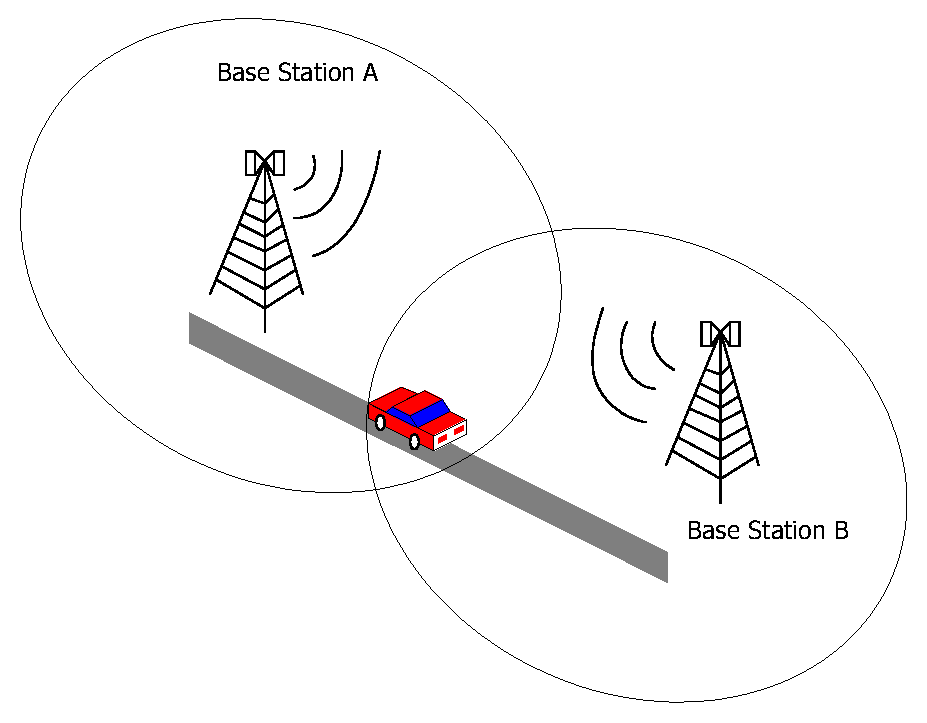
\includegraphics[height=6.75cm]{../figures/iccs_handover_bs}
%\caption{Simulation results of the probability of a handover success using the proposed adaptive FEC scheme.}
\caption{基站切换示意图}
\label{fig:chap_iccs_handover_bs}
\end{centering}
\end{figure}
%%%%%%%%%%%%%%%%%%%%%%%%%%%%%%%%%%%%%%%%%%%%%%%%%%%%%%%%%%%%%%%%%%%%%

当前的移动WiMAX标准详细定义了在切换过程中所需的切换信令协议。
这些协议被用来在单点到多点(Point-to-multipoint,PMP)模式的通信中支持切换过程。
通常,切换技术可以细分成两种:软切换(Soft handover, SHO)和硬切换(Hard Handover,HHO)。
在软切换过程中,移动台在切断与原有基站通信之前,就已经完成和目标基站的切换信令交换过程,并建立了正常的通信连接。
而在硬切换过程中,移动台先要完全断开与原有服务基站的连接,然后再与目标基站建立通信连接。
显然,软切换的优点在于在切换的过程中,数据连接始终存在。
但是同时资源利用率相比硬切换要低。
在硬切换过程中,数据连接会断开一个小的时间段。
因此会引入了一些延时,对于时间敏感的应用而言,需要做专门地处理和优化来确保通信服务质量。
此外,对于时间敏感的应用,软切换也会进行一些优化的处理才能保证在移动WiMAX中用户QoS的体验。


近些年来,对于软切换方面的研究,许多学者做了许多工作。
一部分学者的工作是集中在目标基站的选择策略上。
通过对移动台位置变化的预测、收集分析相邻基站的QoS信息或是对基站信号的分析来优化目标基站的选择\cite{Hsieh:INFOCOM2003}\cite{DooHwan:WPC2006}。
另外一些学者的工作主要是集中在提高一些特定QoS的指标上面。
例如,学者Minsiki为了解决在切换过程中丢包率增加的问题,采用交叉层的设计方法。他们在上层设备中,如网络层中的路由器,缓存切换用户的数据\cite{MinsikICACT2006}。
学者Chen等为了减少切换过程中的延时,提出了一种预协商的机制。
这个机制利用预测移动台与基站间的距离,提前在目标基站中分配所需要的资源\cite{JenHui:AUSWIRELESS:2007}。
学者Ling通过用IP层的链路来传送MAC层的信息来达到减少切换延时的目的\cite{LingVTC2007}。
还有一些学者的研究集中在切换过程中出现的CID(Connection Identifier) 分配冲突,提出了更为合理的分配方案,或是对移动台的数据进行分类处理,也可以提高QoS的水平\cite{Hu:TVT2004}\cite{Wenhua:ICC2007}。


以往的大部分工作主要是从数据链路层或IP层来考虑切换的性能。他们的工作一般是假设无线信道是一个理想信道。在本章中,我们认为如果物理层的信道工作能与数据链路层工作进行协调,就可以有效地提高切换性能。特别是在移动台高速运动的状态下。
下面,我们将会分析信道质量对切换信令交换流程的影响。
然后,通过建立信令交换的概率模型来分析在高速移动状态时的切换性能。
最后通过建立一个简单实用的自适应前向纠错方法来提高切换的成功率和效率。


\section{基站切换成功概率模型}
\label{section_iccs_handover_algorithm_mobility_analysis}
\esection{Probability Model of Handover}
切换的性能与效率通常可以用一个切换的成功率来描述。我们通过统计在切换过程中每次信令的交换成功概率来计算出完成整个切换过程的概率。
在高速运动的切换过程中,移动速度会对切换造成非常大的影响。它不但反映移动台切换延时情况,也在研究切换用户丢包模型中扮演着重要的角色。
\subsection{切换的流程建模分析}
\esubsection{Hanover Protocols in WiMAX}
\label{subsection_iccs_handover_algorithm_mobility_analysis_handover_flow}
在IEEE 802.16e的标准中,切换信令的交换流程如图\ref{fig:chap_iccs_handover_algorithm_handover_flow}所示。
基站会周期地广播“邻近通告消息”(Neighbor Advertisement Message, MOB\_NBR-ADV)。
这个消息用来标识邻近基站或是它们的信道特征。
移动台总是会侦听此消息来收集邻近基站的信息。
如果一个移动台检测到当前服务基站的信道变差,它会发送一个请求消息(MOB\_SCAN-REQ)给当前服务的基站。
如果基站收到这个请求消息后,会反馈给移动台一个消息(MOB\_SCAN-RSP)。
此消息会指示移动台使用特定的无线资源(如时隙)来进行扫描操作(Scanning),确定目标基站。
当扫描操作结束后,移动台初始化切换过程,发送切换请求消息(MOB\_MSHO-REQ)给当前基站。
基站则会发送响应消息信息(MOB\_BSHO-RSP)。
当移动台收到此消息时,它会发送消息(MOB\_HO-IND)通知当前基站可以关闭此移动台的连接,释放无线资源。
(如果是硬切换,移动台会中断与当前服务基站的连接。如果是软切换,连接会继续保留直到与目标基站的信令交换结束。)
最后,移动台与目标基站交换测距消息以及重新接入的各种信令来完成剩余的切换流程。
综合上面的描述,一次成功的切换过程,尽管无线资源的分配也是切换需要考虑的内容,
但从数据链路层的信令层面上看,其核心首先是各种切换信令的成功传递与交换。

%%%%%%%%%%%%%%%%%%%%%%%%%%%%%%%%%%%%%%%%%%%%%%%%%%%%%%%%%%%%%%%%%%%
\begin{figure}[t]
\centering
\includegraphics[height=7.75cm]{iccs_handover}
\caption{切换流程示意图}
%\caption{Illustration of the handover procedure.}
\label{fig:chap_iccs_handover_algorithm_handover_flow}
\end{figure}
%%%%%%%%%%%%%%%%%%%%%%%%%%%%%%%%%%%%%%%%%%%%%%%%%%%%%%%%%%%%%%%%%%%

\subsection{切换成功概率建模与误比特率}
\esubsection{Probability of Handover Success and Bit Error Rate}
根据上面的分析,我们考虑一个这样的切换过程模型。
不失一般性,我们假设在移动台的一次切换过程中有~$M$~($M \ge 2 $)个信令需要交换。
这里用事件~$A_i$~表示一次信令的传送。
 ~$p_i$~是此次信令成功传送的概率,其中 ~$i = 0,1, \cdots, M-1 $~。
如果不考虑自动重传(ARQ)的策略,则得出以下结论:
%%%%%%%%%%%%%%%%%%%%%%%%
\begin{equation}
\label{eq:chap_iccs_handover_algorithm_pro_mess_no_tran}
\begin{cases}
P(A_{i})=p_{i}\\
P(\bar{A}_{i})=1- p_{i}
\end{cases}
\end{equation}
%%%%%%%%%%%%%%%%%%%%%%%%
其中,~$i=0,1,\cdots,M-1$~。
接下来,我们分析一下有重传策略的情况。
在切换过程中,重传策略不但可以用于用户数据的传递,也可用于保证信令消息的可靠传送。
所以,根据切换信令的要求,一个信令消息如果不能被对方成功接收,将会被重传定时器激发重新发送过程,并直到接到对方反馈为止。
那么,如果考虑了重传策略后,则公式 (\ref{eq:chap_iccs_handover_algorithm_pro_mess_no_tran})可以改写为下面的式子:
%%%%%%%%%%%%%%%%%%%%%%%%
\begin{equation}
\label{eq:chap_iccs_handover_algorithm_Pro_basic01}
P(A_{i})=\sum_{j=1}^{N_{i}}q_{i}^{j-1}p_{i}=\sum_{j=1}^{N_{i}}
(1-p_{i})^{j-1}p_{i},\quad N_{i}\geq1,
\end{equation}
%%%%%%%%%%%%%%%%%%%%%%%%
其中,~$N_i$~表示在一次切换过程中,第~$i$~个信令消息在成功接收前被传递的次数。在切换过程中有~$M$~个信令消息,那么,只有~$M$~个信令都成功收到,切换才是成功的,所以一次切换成功的概率可表示为:
%%%%%%%%%%%%%%%%%%%%%%%%%%
\begin{equation}
\label{eq:chap_iccs_handover_algorithm_Pro_basic02}
P_{succ}=\prod_{i=0}^{M-1}P(A_{i})=\prod_{i=0}^{M-1}
\left[\sum_{j=1}^{N_{i}}(1-p_{i})^{j-1}p_{i}\right].
\end{equation}
%%%%%%%%%%%%%%%%%%%%%%%%%%
因为当前通信系统的物理层中普遍采用交织信道编码的技术,所以模型中的无线信道可以假设为无记忆的信道。那么,概率~$p_i$~将主要与移动台和基站之间的无线信道的误比特率有关。我们用数学公式表示如下:
%%%%%%%%%%%%%%%%%%%%%%%%%%
$$
p_{i}=\varphi(P_{b}(\gamma_{b}),\: L_{i}),
$$
%%%%%%%%%%%%%%%%%%%%%%%%%%
其中,~$P_b(\gamma_b)$~是当接收比特信噪比为~$\gamma_b$~的误比特概率。这样,设第~$i$~个信令消息的长度为~$Li$~,则有
%%%%%%%%%%%%%%%%%%%%%%%%
\begin{equation}\label{eq:chap_iccs_handover_algorithm_Pro_basic03}
p_{i}=[1-P_{b}(\gamma_{b})]^{L_{i}}.
\end{equation}
%%%%%%%%%%%%%%%%%%%%%%%%
所以,将公式(\ref{eq:chap_iccs_handover_algorithm_Pro_basic03})代入公式(\ref{eq:chap_iccs_handover_algorithm_Pro_basic02}),可以得到切换模型中的切换成功概率与无线信道误比特率之间的关系。
%%%%%%%%%%%%%%%%%%%%%%%%%
\begin{align}
\label{eq:chap_iccs_handover_algorithm_Pro_basic_final}
\notag P_{succ}&=\prod_{i=0}^{M-1}P(A_{i})\\
&=\prod_{i=0}^{M-1}\left\{ \sum_{j=1}^{N_{i}}\left\{ 1-[1-P_{b}(\gamma_{b})]^{L_{i}}\right\} ^{j-1} \cdot[1-P_{b}(\gamma_{b})]^{L_{i}}\right\}
\end{align}
%%%%%%%%%%%%%%%%%%%%%%%%%%
%%%%%%%%%%%%%%%%%%%%%%%%%%%%%%%%%%%%%%%%%%%%%%%%%%%%%%%%%%%%%%%%%%%%%
\begin{figure}[t]
\begin{centering}
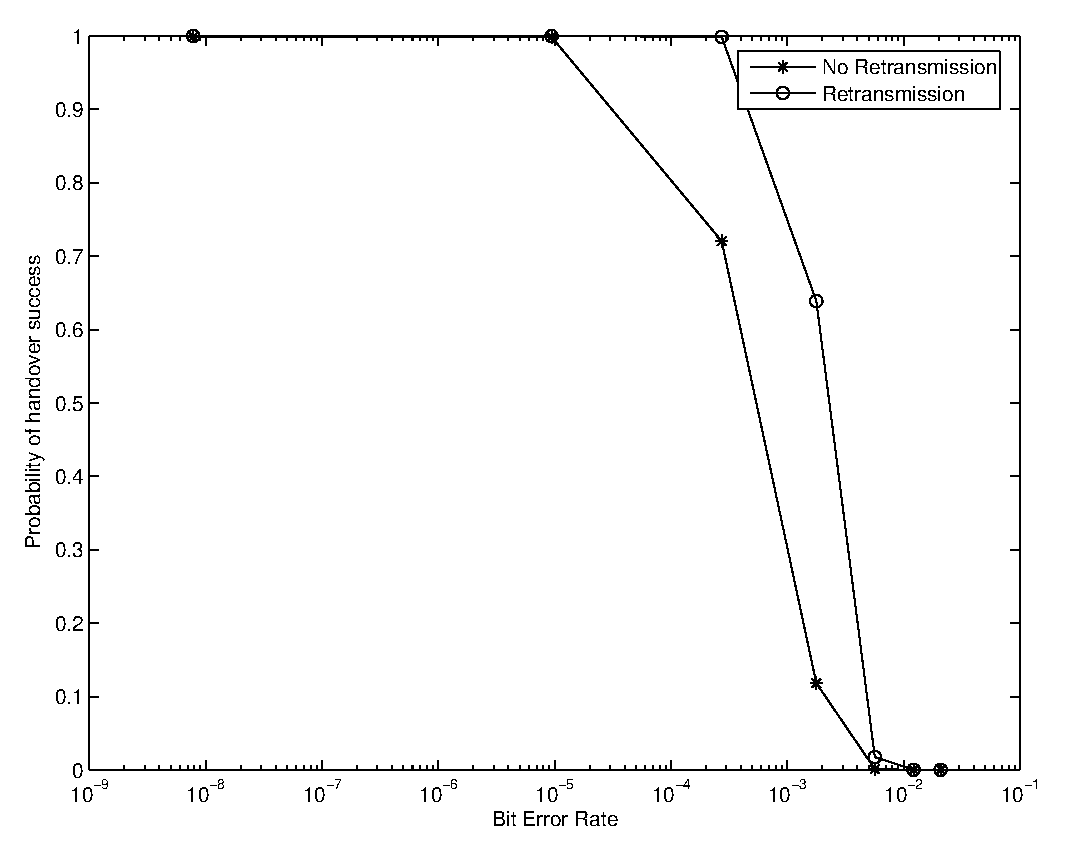
\includegraphics[height=7.75cm]{iccs_ber_prob}
\par\end{centering}
%%\caption{Probability of a handover success as a function of BER, where ~$M=5,\sum_{i=0}^{M-1}N_i<=50,L_i=250$~ bits in this case.}
\caption{切换成功概率与误比特率的关系。在此例中,~$M=5,\sum_{i=0}^{M-1}N_i<=50,L_i=250$~}
\label{fig:chap_iccs_handover_algorithm_PBER}
\end{figure}
%%%%%%%%%%%%%%%%%%%%%%%%%%%%%%%%%%%%%%%%%%%%%%%%%%%%%%%%%%%%%%%%%%%%%
这里,我们给出公式(\ref{eq:chap_iccs_handover_algorithm_Pro_basic_final})的一个例子,如图 \ref{fig:chap_iccs_handover_algorithm_PBER} 所示。
可以明显地看出,对于固定的~$N_i$~,切换的成功概率~$P_{succ}$~随着误比特概率~$P_b(\gamma_b)$~的增大而降低。当误比特率较大时(在~$10^{-4}$~到~$10^{-2}$~之间),使用重传策略会有效地改善切换的成功率。

\subsection{切换成功概率模型与移动台速度}
\esubsection{Probability of Handover Success and Velocity of MS}
上一节的分析指出了切换成功概率与两个重要的参数有关:一是信道的误比特率,二是信令消息的重传次数。
在一个实际的WiMAX网络中,这二者都与移动台的移动速度有关。
首先,移动的速度会影响多谱勒频率偏移,进而影响信道的误比特率,最终对信令消息的重传次数产生影响。
其次,两个相邻基站信号覆盖的交叠部分的物理距离有限,因而不能做到无限次数的重传。
所以,一个快速移动的终端要求基站切换的速度与时间也有更严格的要求。
基于上述的考虑可知,通常情况下,移动台的移动速度越快,切换成功的概率会越低。

为了定量的分析起见,我们假设在切换过程中,
对信令处理的时间可以忽略不计。
%对时间的影响主要由重传时间间隔引起。
那么,
在整个切换过程中的延时可以定义为下面的式子,
%%%%%%%%%%%%%%%%%%%%%%%%%%%%%%%%%%%%%
$$
T_{M}=(N_{0}+N_{1}+\cdots+N_{M-1})\cdot T_{retx}+M\cdot T_{prop},
$$
%%%%%%%%%%%%%%%%%%%%%%%%%%%%%%%%%%%%%
其中,~$N_i$~表示第~$i$~个信令传递的次数。~$T_{retx}$~是同一信令消息重传的计时器间隔,~$T_{prop}$~是在移动台与基站之间承载信令的电磁波传播所需时间。

我们用~$D_{overlap}$~表示在移动台移动方向上两个相邻基站覆盖范围重叠部分的最大距离。
如图\ref{fig:chap_iccs_handover_bs}如示。
$v_m$是移动台的移动速度。
因此,在一次成功的基站切换过程中,需要满足下面的时间约束,如\eqref{eqn:chap_handover:times_T_M}所示:
%%%%%%%%%%%%%%%%%%%%%%%%%%%%%%%%
\begin{equation}
T_{M}<\frac{D_{overlap}}{v_{m}}.
\label{eqn:chap_handover:times_T_M}
\end{equation}
%%%%%%%%%%%%%%%%%%%%%%%%%%%%%%%
在这个约束下,一次成功切换的概率可以进一步被改写为\eqref{eq:chap_iccs_handover_algorithm_Pro_basic_final00},

%%%%%%%%%%%%%%%%%%%%%%%
\begin{equation}
P_{succ}=\left\{
\begin{array}{ll}
\prod_{i=0}^{M-1}\left[\sum_{j=1}^{N_{i}}(1-p_{i})^{j-1}p_{i}\right],
& \mbox{if }T_{M}<\frac{D_{overlap}}{v_{m}},\\
\\0, & \mbox{others},
\end{array}\right.\label{eq:chap_iccs_handover_algorithm_Pro_basic_final00}
\end{equation}
%%%%%%%%%%%%%%%%%%%%%%%
其中,
%%%%%%%%%%%%%%%%%%%%%%%%
\begin{align*}
T_{M}=\sum_{i=0}^{M-1}(N_{i})\cdot T_{retx}+M\cdot T_{prop} \\
p_{i}=[1-P_{b}(\gamma_{b})]^{L_{i}}
\end{align*}
%%%%%%%%%%%%%%%%%%%%%%%%
假设通信信道为Rayleigh信道,平均接收符号的信噪比(energy-to-noise)可以表示为:\cite{GLST:PMC2002}\cite{Leung:WCNC2005}
%%%%%%%%%%%%%%%%%%%%%%%%
\begin{equation}
\bar{\gamma}_{s}=\frac{1}{1-\frac{1}{N^{2}}\left[N+2\sum_{i=1}^{N-1}\left(N-i\right)J_{0}(2\pi f_{m}T_{s}i) \right]
+\frac{NT_{s}}{E_s/N_{0}}},
\end{equation}
%%%%%%%%%%%%%%%%%%%%%%%
其中,~$N$~是OFDM子载波的个数,~$T_s$~是一个K阶QAM调制的符号在一个子载波上的传输时间。~$N_0$~是噪声功率, ~$E_s$~是传送每个符号的平均能量。~$f_{m}=fv_{m}/c $~是最大的多谱勒频偏,~$f$~为载波频率,~$v_m$~为移动台的速度,~$c$~为光速。那么相应的接收到的平均比特信噪比为
%%%%%%%%%%%%%%%%%%%%%%%%
\begin{align}
\bar{\gamma}_{b}&= \frac{ \bar{\gamma}_s} {\log_2K} \notag\\
&=\frac{1/\log_{2}K}{1-\frac{1}{N^{2}}\left[N+2\cdot \sum_{i=1}^{N-1}\left(N-i\right) J_{0}(2\pi f_{m}T_{s}i) \right]
+\frac{NT_{s}}{\log_{2}K}\left(\frac{1}{E_{b}/N_{0}}\right)}
\label{eqn:chap_handover:avg_snr}
\end{align}
其中,
\begin{equation*}
J_{0}(2\pi f_{m}T_{s}i) = \frac{1}{\pi}\int_0^\pi \cos(2\pi f_m T_{s}i \sin \theta) d \theta
\end{equation*}
%%%%%%%%%%%%%%%%%%%%%%%
此处,我们假设以Clarke-Jakes的模型为基础的Rayleigh信道模型。

%其中,~$Y$~定义为
%%%%%%%%%%%%%%%%%%%%%%%%
%$$
%Y=\sum_{i=1}^{N-1}\left(N-i\right)J_{0}(2\pi f_{m}T_{s}i)
%$$
%%%%%%%%%%%%%%%%%%%%%%%%%
对于K阶的QAM调试(如果~$K=4$~,调制的方式是QPSK;如果~$K=16$~,那么就是16-QAM)。
我们假设在接收端可以进行出错的符号检测。那么对于当接收比特能量与噪声比为~$\gamma_b$~时,误比特概率(bit error, BER)为~$P_b(\gamma_b)$~可以写为:
%%%%%%%%%%%%%%%%%%%%%%%
\[
{{P}_{b}}=\int\limits_{0}^{\infty }{{{P}_{b}}(\gamma ){{f}_{{{\gamma }_{b}}}}(}\gamma )d\gamma
\]
%%%%%%%%%%%%%%%%%%%%%%%%
其中,~$f_{\gamma_b}$~是Rayleigh信道模型的比特能量与噪声比的概率密度函数。它定义如下:
%%%%%%%%%%%%%%%%%%%%%%%%%
\[{{f}_{{{\gamma }_{b}}}}(\gamma )=\frac{\exp (\frac{-\gamma }{{{{\bar{\gamma }}}_{b}}})}{{{{\bar{\gamma }}}_{b}}},\gamma \ge 0\]
%%%%%%%%%%%%%%%%%%%%%%%%%%%%
我们假设载波间的干扰(ICI)为高斯白噪声。这个值近似在~$256 \le N \le 1024$~是比较精确的\cite{Leung:WCNC2005}。那么,对于K阶的QAM和Gray码,可以有如下的近似,
%%%%%%%%%%%%%%%%%%%%%%%
\begin{equation}
P_b(\gamma_b) \approx \frac{P_K(\gamma_s)}{\log_2 K}
\end{equation}
%%%%%%%%%%%%%%%%%%%%%%%
其中,~$P_K$~是符号的错误概率。特别对于QPSK,有
%%%%%%%%%%%%%%%%%%%%%%%%
\begin{align}
\label{eq:chap_iccs_handover_algorithm_BER_V}
P_{b}(\gamma_{b})&= Q\left(\sqrt{2\gamma_{b}}\right).\\
Q(x) &= \int^x_{-\infty} \frac{1}{\sqrt{2\pi}}e^{-y^2/2}dy \notag
\end{align}
%%%%%%%%%%%%%%%%%%%%%%%%
把公式(\ref{eq:chap_iccs_handover_algorithm_Pro_basic_final00})和公式( \ref{eq:chap_iccs_handover_algorithm_BER_V})合并则有下面的结果。
%%%%%%%%%%%%%%%%%%%%%%%
\begin{equation}
P_{succ}=\left\{
\begin{array}{ll}
\prod_{i=0}^{M-1}\left[\sum_{j=1}^{N_{i}}(1-Q\left(\sqrt{2\gamma_{b}}\right))^{j-1}Q\left(\sqrt{2\gamma_{b}}\right)\right],
& \mbox{if }T_{M}<\frac{D_{overlap}}{v_{m}},\\
\\0, & \mbox{others}
\end{array}\right.\label{eq:chap_handover:velocity_bit_error_rate}
\end{equation}
其中,~$\gamma_b$~是移动速度的一个函数。
至此,我们可以得到以移动台速度为变量的一个切换成功概率函数模型。其函数图形,如图\ref{fig:chap_iccs_handover_algorithm_Pro_V} 所示。
%%%%%%%%%%%%%%%%%%%%%%%%%%%%%%%%%%%%%%%%%%%%%%%%%%%%%%%%%%%%%%%%%%%%
\begin{figure}[t]
\begin{centering}
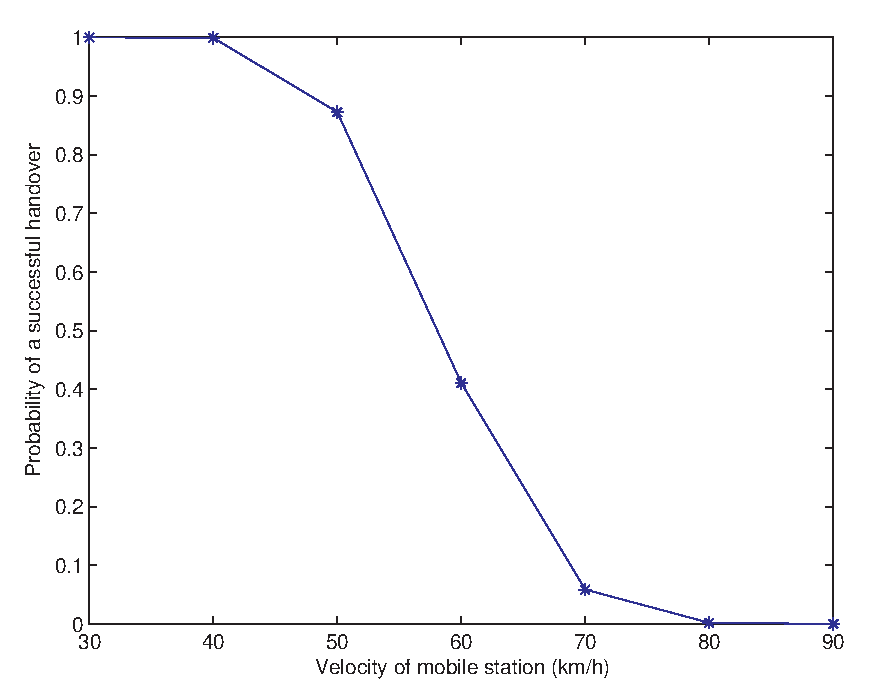
\includegraphics[height=7.75cm]{iccs_speed_prob_theroy}
%%\caption{The probability of a handover success as a function of MS's velocity, where ~$M=5, \sum_{i=0}^{M-1}N_i=50, L_i=250$~ bits in this case.}
\caption{切换成功概率与用户的移动速度关系,在本例中~$M=5, \sum_{i=0}^{M-1}N_i=50, L_i=250$~}
\label{fig:chap_iccs_handover_algorithm_Pro_V}
\end{centering}
\end{figure}
%%%%%%%%%%%%%%%%%%%%%%%%%%%%%%%%%%%%%%%%%%%%%%%%%%%%%%%%%%%%%%%%%%%%

从图中可明显看出,随着移动的速度增快,切换成功概率会显著下降。速度很大程度上影响了切换的过程。所以说,如果在高速移动状态下,切换对于移动台来说需要额外的处理措施。

\section{基于切换成功概率模型的切换方案}
\esection{Handover Scheme with High Velocity MS}
在高速移动状态下,为了提高移动台的切换成功概率,除了可以减小重传间隔、增加重传的次数以外,我们还可以建立更加可靠的通信链路的传输机制来传送信令消息。
本节我们讨论了前向纠错编码的特点,并采用此技术来改善传输的误码率。
前向纠错编码是通过发送端使用冗余比特数来提供差错保护。
这些额外的冗余比特可以帮助接收端检测并纠正错误。
如果采用了前向纠错的技术,数据重传的次数也会降低。
%根据WiMAX的标准,切换信令的消息大小约为50到180个字节。

不同的前向纠错编码方案可以提供不同的纠错能力。
对于同一种前向纠错码而言,冗余比特数越多,纠错能力也超强。
同时由于无线信道的限制及交换的信令消息较多,所以要在满足设计要求的基础上尽可能减少冗余比特数。

下面,我们定量地讨论冗余比特的个数。对于一个给定的移动台速度,我们要能根据系统设计要求达到的切换成功率来计算出冗余比特数。为了简单起见,我们使用切换消息信令的平均长度,设切换消息传输一次的成功的概率为~$\tilde{p}$~以替换公式(\ref{eq:chap_iccs_handover_algorithm_Pro_basic_final00})中的~$p_i$~,如下
%%%%%%%%%%%%%%%%%%%%%%%%%%%%%%%%%%%
\begin{align}
\notag P_{succ} &= \prod_{i=0}^{M-1}P(A_{i})\\
&= \prod_{i=0}^{M-1}\left[\sum_{j=1}^{N_{i}}(1-p_{i})^{j-1}p_{i}\right]\\
\notag &\thickapprox\sum_{i=M}^{S}{i-1 \choose M-1}\cdot\widetilde{p}^{M}(1-\widetilde{p})^{i-M}
\end{align}
%%%%%%%%%%%%%%%%%%%%%%%%%%%%%%%%%%
其中,~$S=\sum_{i=0}^{M-1}N_{i}$~是总共重传的次数。根据前面小节的分析,可以得到如下的公式:
%%%%%%%%%%%%%%%%%%%%%%%%%%%%%%%%%%
\begin{align*}
S & = \sum_{i=0}^{M-1}N_{i}\\
  & = \left\lfloor \frac{(\frac{D_{overlap}}{v_{m}}-MT_{prop})}
        {T_{retx}}\right\rfloor \leq\frac{(\frac{D_{overlap}}{v_{m}}
        -MT_{prop})}{T_{retx}}.
\end{align*}
%%%%%%%%%%%%%%%%%%%%%%%%%%%%%%%%%%
这样,我们就可根据相邻基站覆盖交叠的距离~$D_{overlap}$~和移动台的速度~$v_m$~,得到参数~$S$~;并根据系统设计要求的~$P_{succ}$~进一步计算得每一个信令的成功传输的概率值。如果使用Reed-Solomon(R-S)纠错编码,我们可以推导出如下 \eqref{eq:chap_iccs_handover_algorithm_FEC_Pro_final}。
%%%%%%%%%%%%%%%%%%%%%%%%%%%%%
\begin{equation}\label{eq:chap_iccs_handover_algorithm_FEC_Pro_final}
\tilde{p}\approx\frac{2^{k-1}}{k(2^{k}-1)^{2}}\sum_{j=t+1}^{2^{k}-1}j
\cdot{2^{k}-1\choose j}_{}^{}\cdot p^{j}(1-p)^{2^{k}-1-j},
\end{equation}
%%%%%%%%%%%%%%%%%%%%%%%%%%%%%
其中, ~$t=\lfloor\frac{N-k}{2}\rfloor$~ 是编码的符号纠错能力,~$N$~是全部的比特数,~$k$~是信令消息的比特数, ~$\lfloor{x}\rfloor$~表示不超过~$x$~的最大整数。那么冗余比特数~$N-k$~可以确定下来。图 \ref{fig:chap_iccs_handover_algorithm_AFEC_bits} 表明了在切换流程要达到不同的切换成功概率(~$50\%,80\%,99\%$~)时,在不同的速度下,移动台切换所需的冗余比特数。
%%%%%%%%%%%%%%%%%%%%%%%%%%%%%%%%%%%%%%%%%%%%%%%%%%%%%%%%%%%%%%%%%%%%%%%%%%%
\begin{figure}[t]
\begin{centering}
\includegraphics[height=6.75cm]{iccs_speed_size_theory}
\caption{RS码中的冗余比特数与移动台速度之间的关系,其中,假设~$k=250$~比特}
\label{fig:chap_iccs_handover_algorithm_AFEC_bits}
\end{centering}
\end{figure}
%%%%%%%%%%%%%%%%%%%%%%%%%%%%%%%%%%%%%%%%%%%%%%%%%%%%%%%%%%%%%%%%%%%%%%%%%%%

如图 \ref{fig:chap_iccs_handover_algorithm_AFEC_bits}所示,当移动台的速度越快,那么为了要达到系统设定的切换成功概率,所需的冗余比特数也越多。例如,为了能够达到~$80\%$~的成功概率,如果移动台的速度分别是50,70, 90 km/h,那么所需的冗余比特数是2,10,28。通过上面的分析,我们可以使用一种自适应的方法根据不同的移动台速度来增加所需的冗余比特。

\section{仿真实验与结果分析}
\esection{Simuation and Results}
我们通过计算机仿真实验来验证和评估我们的切换概率模型及相应的前向纠错方案。在实验中,我们使用了NS-2仿真模拟器和修改了的NIST的WiMAX仿真代码\cite{NS2_simulator}\cite{NIST_WIMAX}。仿真实验中主要的实验设置参数如表格\ref{chap_iccs_table_I} 所示。

%%%%%%%%%%%%%%%%%%%%%%%%%%%%%%%%%%%%%%%%%%%%%%%%%%%%%%%%%%%%%%%%%%%%%
\begin{table}[htbp]
\wuhao
\centering
%\begin{centering}
\caption{仿真实验的主要参数配置}\label{chap_iccs_table_I}
\begin{tabular*}{0.99\textwidth}{p{7cm} p{7cm}} 
\toprule 
参数名称  & 参数值 \\
\midrule
移动方向上的交叠距离  & 200 米\tabularnewline 
带宽  & 5 MHz\tabularnewline 
载波频率  & 2.5 GHz\tabularnewline 
FFT   & 512\tabularnewline
信道类型  & Rayleigh channel\tabularnewline 
FEC  & Reed-Solomon code\tabularnewline 
移动速度  & 30-90 km/h\\
\bottomrule
\end{tabular*}
%\end{centering}
\end{table}
%%%%%%%%%%%%%%%%%%%%%%%%%%%%%%%%%%%%%%%%%%%%%%%%%%%%%%%%%%%%%%%%%%%%%

这里,我们采用的是自适应的前向纠错码方案。
冗余比特数是理论计算事先得到的。
在切换成功概率为50\%,80\%,99\%的情况下,计算出所需要的冗余比特数。
对于每一组实验参数,仿真进行100次,然后取结果的平均值来得到最后的统计结果。
最终得到的仿真实验结果,如\figref{fig:chap_iccs_results}所示。
从图中我们可以看到,在移动台的速度较低时,少量增加一些冗余比特会使得切换成功的概率会显著增加,并接近于~1。
而当速度逐渐增大后,对于目标为50\%的曲线,切换成功率会下降,但仍然会保持在50\%以上。
这说明,为保证较高的切换成功率,如99\%,所增加的冗余比特数较多,我们的方案略显些保守。
而且我们也注意到,在速度为70km/h时,理论成功率50\%的曲线存在一个局部极值点。
经过反复实验与比对,我们认为有两个原因会造成:
一是,在NS2系统中的Rayleigh信道模型计算误比特数时存在偏差。
二是,\eqref{eqn:chap_handover:avg_snr}中速度与SNR关系偏差所致。

%%%%%%%%%%%%%%%%%%%%%%%%%%%%%%%%%%%%%%%%%%%%%%%%%%%%%%%%%%%%%%%%%%%%%
\begin{figure}[t]
\begin{centering}
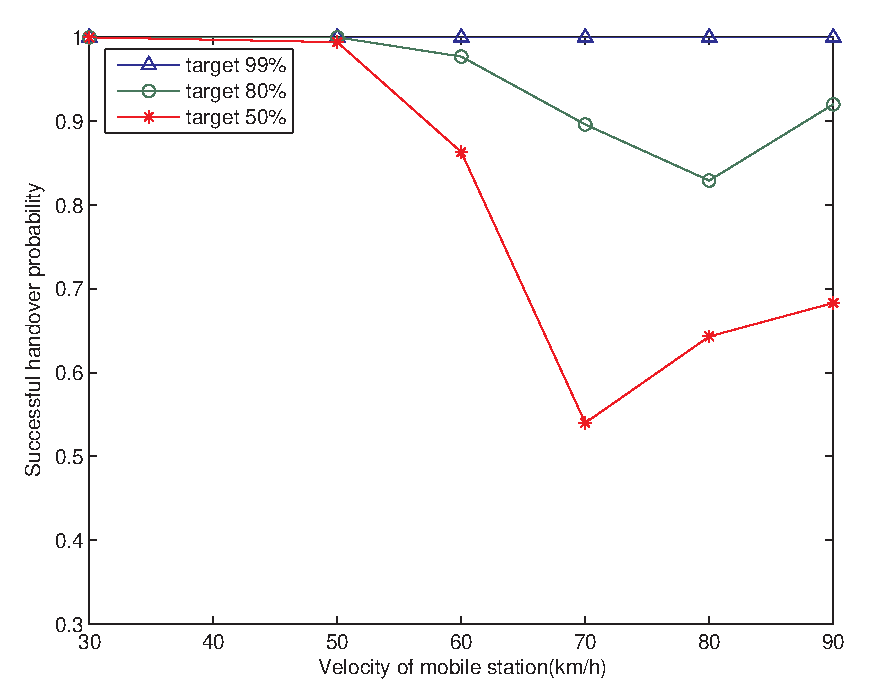
\includegraphics[height=7.75cm]{iccs_speed_prob_simu}
%\caption{Simulation results of the probability of a handover success using the proposed adaptive FEC scheme.}
\caption{仿真实验的结果}
\label{fig:chap_iccs_results}
\end{centering}
\end{figure}
%%%%%%%%%%%%%%%%%%%%%%%%%%%%%%%%%%%%%%%%%%%%%%%%%%%%%%%%%%%%%%%%%%%%%

\section{本章小结}
\esection{Chapter Summary}
在本章中,我们以WiMAX网络为例分析了移动台的移动速度对切换成功率的影响。分析的结果表明,由于移动台的速度增加会导致无线传输的信道变差,进而使得切换信令不能正常收发。又由于切换操作是时间受限的,所以在设计切换时要两方面同时考虑。根据理论分析,我们提出了一个简单有效的自适应前向纠错方案,通过理论计算就可以得到在不同速度下所需的冗余比特数,可以满足在不同移动速度下的切换设计需求。最后仿真实验验证了我们的理论模型和所提出的前向纠错方案的正确性。
%chapter_end
